\documentclass[11pt,a4paper]{article}
\usepackage[utf8]{inputenc}
\usepackage[margin=1in]{geometry}
\usepackage{mathpazo}
\usepackage{booktabs}
\usepackage{graphicx}
\usepackage{xcolor}
\usepackage{hyperref}
\usepackage{enumitem}
\usepackage{tikz}
\usepackage{pgfplots}
\usetikzlibrary{positioning}
\usepackage{tcolorbox}
\usepackage{tabularx}
\usepackage{array}
\pgfplotsset{compat=1.18}
\tcbuselibrary{skins, breakable}

\definecolor{reviewgreen}{HTML}{5D8057}
\definecolor{reviewsand}{HTML}{B2986E}
\definecolor{reviewred}{HTML}{A86464}
\definecolor{reviewblue}{HTML}{6E8AA4}
\definecolor{reviewpurple}{HTML}{9B8FAF}
\definecolor{reviewgray}{HTML}{8A8A8A}
\definecolor{bgwarm}{HTML}{FAF8F5}
\definecolor{textdark}{HTML}{3A3A3A}

\newcommand{\scorecolor}[1]{%
  \ifnum#1>7 \textcolor{reviewgreen}{\textbf{#1/10}}%
  \else\ifnum#1>4 \textcolor{reviewsand}{\textbf{#1/10}}%
  \else \textcolor{reviewred}{\textbf{#1/10}}%
  \fi\fi}

\newcommand{\scorebar}[1]{%
  \begin{tikzpicture}[baseline=-0.5ex]
    \fill[reviewgray!20] (0,0) rectangle (2.5,0.3);
    \ifnum#1>7
      \fill[reviewgreen!60] (0,0) rectangle ({#1*0.25},0.3);
    \else\ifnum#1>4
      \fill[reviewsand!60] (0,0) rectangle ({#1*0.25},0.3);
    \else
      \fill[reviewred!60] (0,0) rectangle ({#1*0.25},0.3);
    \fi\fi
    \draw[reviewgray!40] (0,0) rectangle (2.5,0.3);
  \end{tikzpicture}%
}

\newtcolorbox{originaltext}{
  colback=reviewred!6, colframe=reviewred!50,
  fonttitle=\bfseries\small, title=Original Text,
  left=10pt, right=10pt, top=6pt, bottom=6pt,
  boxrule=0.8pt, arc=4pt, breakable,
  shadow={1pt}{-1pt}{0pt}{reviewgray!15}
}
\newtcolorbox{revisedtext}{
  colback=reviewgreen!6, colframe=reviewgreen!50,
  fonttitle=\bfseries\small, title=Suggested Revision,
  left=10pt, right=10pt, top=6pt, bottom=6pt,
  boxrule=0.8pt, arc=4pt, breakable,
  shadow={1pt}{-1pt}{0pt}{reviewgray!15}
}
\newtcolorbox{insightbox}[1][]{
  colback=reviewblue!6, colframe=reviewblue!50,
  fonttitle=\bfseries\small, title={#1},
  left=10pt, right=10pt, top=6pt, bottom=6pt,
  boxrule=0.8pt, arc=4pt, breakable
}

\hypersetup{
  colorlinks=true,
  linkcolor=reviewblue,
  urlcolor=reviewblue,
  citecolor=reviewgreen,
}

\title{\textcolor{textdark}{Academic Review Report}}
\author{AI Reviewer}
\date{\today}

\begin{document}
\maketitle

\section{Executive Summary}
This paper introduces Group Bias Adaptation (GBA) for sparse autoencoders (SAEs) and pairs it with the first provable feature-recovery guarantee for a simplified SAE training regime. The strongest aspect is the technical core: epsilon-identifiability (Theorem 5.3) and a detailed dynamics analysis (Theorem 6.1) with synthetic experiments that directly test the theory's key predictions. The main concern is the theory-practice gap and incomplete empirical positioning (missing JumpReLU-SAE baseline and downstream utility evaluation), but these appear fixable in revision.

\begin{insightbox}[Verdict at a Glance]
\begin{tabular}{lrl}
\textbf{Overall Score:} & \textcolor{reviewsand}{\textbf{6.85/10}} & \scorebar{7} \\
\textbf{Recommendation:} & \multicolumn{2}{l}{\textit{Accept (NeurIPS 2025), conditional on revisions}} \\
\textbf{Confidence:} & \multicolumn{2}{l}{\textit{Medium}} \\
\end{tabular}
\end{insightbox}

\section{Document Overview}
\begin{tabularx}{\textwidth}{>{\bfseries}lX}
Title & Taming Polysemanticity in LLMs: Provable Feature Recovery via Sparse Autoencoders \\
Authors & Siyu Chen, Heejune Sheen, Xuyuan Xiong, Tianhao Wang, Zhuoran Yang \\
Affiliations & Yale University, Shanghai Jiao Tong University, TTIC \\
arXiv & 2506.14002v1 (June 16, 2025) \\
Target Venue Context & NeurIPS 2025 review standard \\
Length & 133 pages (35 main + references + appendices) \\
\end{tabularx}

\subsection*{Abstract-Level Summary}
The paper formalizes SAE feature recovery using $X=HV$ and proposes epsilon-identifiability to capture permutation, scaling, and feature-splitting ambiguities. It introduces GBA, which adapts neuron biases to hit target activation frequencies while grouping neurons across exponentially decaying frequency bands. Theoretical analysis proves recovery for a simplified Modified BA regime under explicit width/bias/balance conditions, and LLM experiments on Qwen2.5-1.5B show GBA is competitive with TopK on the sparsity-loss frontier and stronger than TopK on cross-seed consistency.

\subsection*{Core Contributions (4)}
\begin{enumerate}[leftmargin=*]
\item Epsilon-identifiability framework for SAE feature recovery under superposition.
\item GBA algorithm: decoupled sparsity control (bias adaptation) + multi-scale grouping.
\item First provable SAE feature-recovery guarantee (Theorem 6.1, simplified setting).
\item Empirical validation on LLM activations and synthetic settings aligned to theory.
\end{enumerate}

\begin{insightbox}[Steel-Man Interpretation]
At its strongest, this work reframes SAE training from ``optimize one objective and hope sparsity emerges'' to ``control sparsity directly while optimizing reconstruction,'' which is a cleaner algorithmic decomposition. The identifiability theorem is model-free and stands independently of dynamics assumptions. The dynamics theorem is restrictive but technically substantial and unusually transparent about its assumptions, while synthetic experiments explicitly test the predicted co-occurrence, bias-range, and width regimes rather than relying only on aggregate benchmark plots.
\end{insightbox}

\section{SAE Background \& Related Work}
\subsection*{Training-Method Landscape}
\begin{itemize}[leftmargin=*]
\item \textbf{L1 SAE}: robust and simple but prone to activation shrinkage and regularization tuning sensitivity.
\item \textbf{TopK SAE}: strong sparsity-loss frontier but high seed sensitivity and fixed-$K$ rigidity.
\item \textbf{JumpReLU SAE}: strong empirical results with learned thresholds, but non-smooth optimization and estimator-tuning overhead.
\item \textbf{GBA (this paper)}: decouples sparsity from reconstruction via bias adaptation; adds neuron groups for multi-frequency features.
\end{itemize}

\subsection*{Theoretical Lineage}
The work builds on sparse dictionary learning and identifiability literature (Olshausen \& Field 1996; Spielman et al. 2012; Arora et al. 2014; Cohen \& Gillis 2019), then connects to modern SAE interpretability practice (Bricken et al. 2023; Gao et al. 2024; Templeton et al. 2024; Rajamanoharan et al. 2024). Its main novelty is not the $X=HV$ model itself, but the SAE-specific identifiability formulation and proof-backed training-dynamics framing.

\subsection*{Comparison Table}
\begin{tabularx}{\textwidth}{p{2.2cm}p{2.2cm}p{2.2cm}p{2.5cm}X}
\toprule
\textbf{Method} & \textbf{Sparsity Mechanism} & \textbf{Key Hyperparams} & \textbf{Known Strength} & \textbf{Key Limitation} \\
\midrule
L1 & Penalty term on activations & $\lambda$ & Stable cross-seed behavior & Shrinkage; weaker sparsity-loss frontier \\
TopK & Hard top-$K$ selection & $K$ & Strong frontier performance & Seed sensitivity; global fixed sparsity \\
JumpReLU & Learned threshold gating & Threshold init, pseudo-deriv tuning & Strong prior SOTA reports & Not included as standalone baseline in this paper's main Fig. 3 \\
GBA & Bias adaptation + group TAFs & $K, p_1, p_K$ (robust regime) & Theory-guided design + good consistency vs TopK & Theory proven for simplified variant, not full deployed algorithm \\
\bottomrule
\end{tabularx}

\section{Argument Flow Analysis}
\subsection*{Logical Structure (TikZ Reconstruction)}
\begin{center}
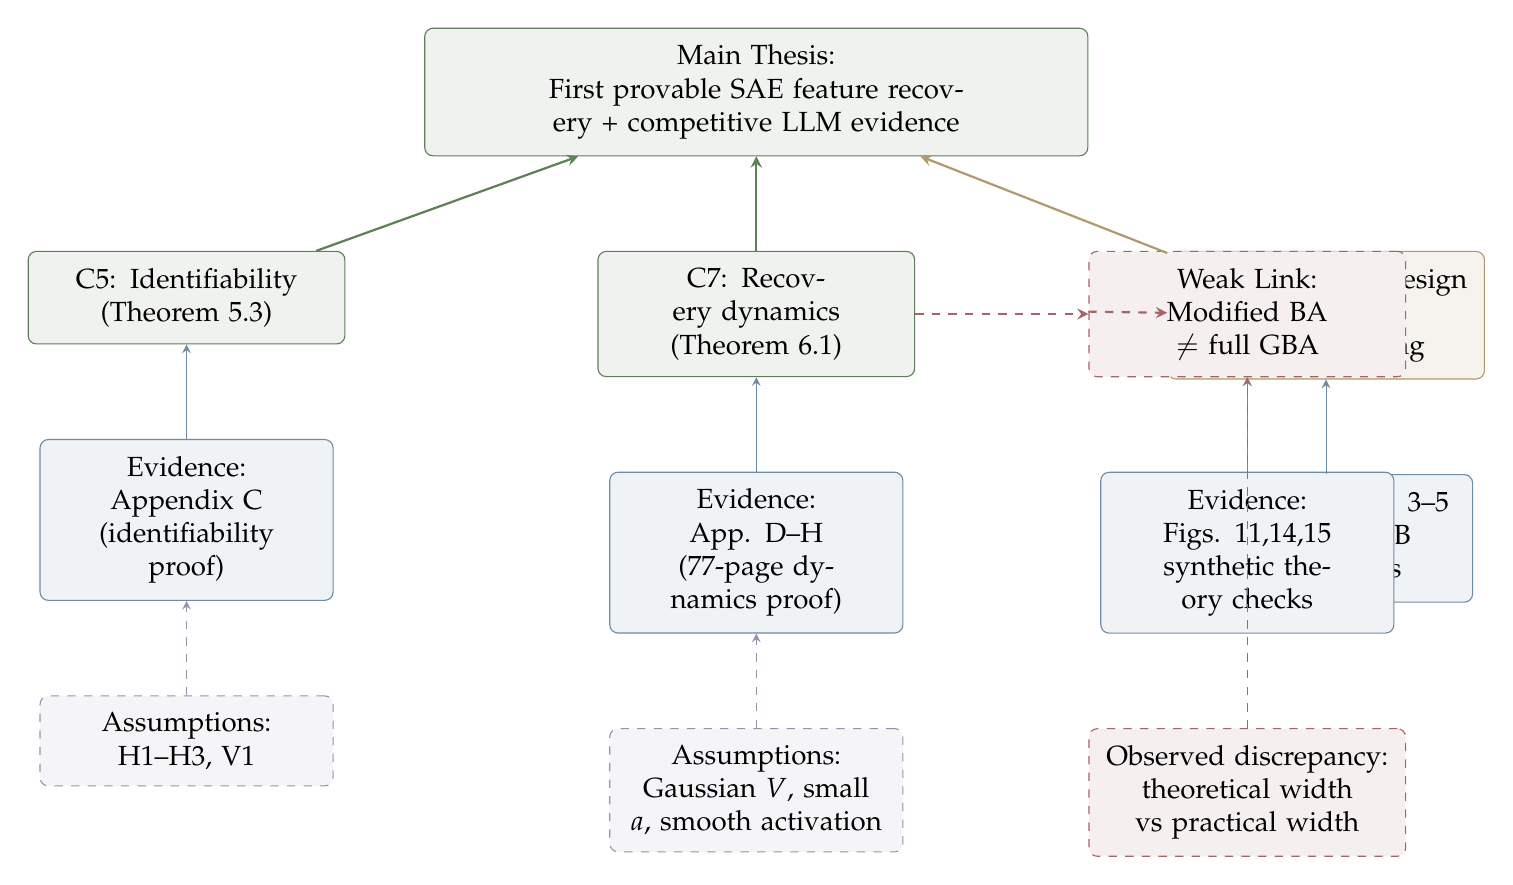
\begin{tikzpicture}[
  >=stealth,
  node distance=1.2cm and 1.0cm,
  claimS/.style={draw=reviewgreen, fill=reviewgreen!10, rounded corners=3pt, align=center, inner sep=6pt, text width=3.6cm},
  claimM/.style={draw=reviewsand, fill=reviewsand!12, rounded corners=3pt, align=center, inner sep=6pt, text width=3.6cm},
  claimW/.style={draw=reviewred, fill=reviewred!10, rounded corners=3pt, dashed, align=center, inner sep=6pt, text width=3.6cm},
  evidence/.style={draw=reviewblue, fill=reviewblue!10, rounded corners=3pt, align=center, inner sep=6pt, text width=3.3cm},
  assume/.style={draw=reviewpurple, fill=reviewpurple!10, rounded corners=3pt, dashed, align=center, inner sep=6pt, text width=3.3cm}
]
\node[claimS, text width=8.0cm] (thesis) {Main Thesis:\\First provable SAE feature recovery + competitive LLM evidence};
\node[claimS, below left=of thesis] (id) {C5: Identifiability\\(Theorem 5.3)};
\node[claimS, below=of thesis] (dyn) {C7: Recovery dynamics\\(Theorem 6.1)};
\node[claimM, below right=of thesis] (gba) {C11/C12: GBA design\\bias adaptation + grouping};
\node[claimW, right=of dyn, xshift=1.2cm] (gap) {Weak Link:\\Modified BA $\neq$ full GBA};

\node[evidence, below=of id] (proofc) {Evidence: Appendix C\\(identifiability proof)};
\node[evidence, below=of dyn] (proofd) {Evidence: App. D--H\\(77-page dynamics proof)};
\node[evidence, below=of gba] (emp) {Evidence: Figs. 3--5\\Qwen2.5-1.5B experiments};
\node[evidence, below=of gap] (syn) {Evidence: Figs. 11,14,15\\synthetic theory checks};

\node[assume, below=of proofc] (a1) {Assumptions: H1--H3, V1};
\node[assume, below=of proofd] (a2) {Assumptions: Gaussian $V$, small $a$, smooth activation};
\node[claimW, below=of syn] (a3) {Observed discrepancy:\\theoretical width vs practical width};

\draw[->, thick, color=reviewgreen] (id) -- (thesis);
\draw[->, thick, color=reviewgreen] (dyn) -- (thesis);
\draw[->, thick, color=reviewsand] (gba) -- (thesis);
\draw[->, thick, dashed, color=reviewred] (dyn) -- (gap);
\draw[->, thick, dashed, color=reviewred] (gap) -- (gba);

\draw[->, color=reviewblue] (proofc) -- (id);
\draw[->, color=reviewblue] (proofd) -- (dyn);
\draw[->, color=reviewblue] (emp) -- (gba);
\draw[->, color=reviewblue] (syn) -- (gap);

\draw[->, dashed, color=reviewpurple] (a1) -- (proofc);
\draw[->, dashed, color=reviewpurple] (a2) -- (proofd);
\draw[->, dashed, color=reviewred] (a3) -- (gap);
\end{tikzpicture}
\end{center}

\subsection*{Coherence Assessment}
Strongest links are the identifiability track (C5) and its proof path, plus direct synthetic validation of key theory conditions. The central weak link is transfer from proven Modified BA assumptions ($a\to0$, fixed bias, smooth activation, single group) to practical GBA ($a=1$, adaptive bias, JumpReLU, multi-group, AdamW). The argument is coherent overall, but empirical claims should be more tightly calibrated to this bridge.

\section{Scoring Dashboard}
\begin{tabular}{lccl}
\toprule
\textbf{Dimension} & \textbf{Weight} & \textbf{Score} & \textbf{Visual} \\
\midrule
Novelty \& Originality & 20\% & \scorecolor{7} & \scorebar{7} \\
Technical Quality & 20\% & \scorecolor{8} & \scorebar{8} \\
Significance \& Impact & 15\% & \scorecolor{7} & \scorebar{7} \\
Clarity \& Presentation & 10\% & \scorecolor{7} & \scorebar{7} \\
Experimental Rigor & 15\% & \scorecolor{5} & \scorebar{5} \\
Reproducibility & 5\% & \scorecolor{7} & \scorebar{7} \\
Literature Coverage & 10\% & \scorecolor{7} & \scorebar{7} \\
Ethical Considerations & 5\% & \scorecolor{6} & \scorebar{6} \\
\midrule
\textbf{Overall (Weighted)} & & \textbf{6.85/10} & \\
\bottomrule
\end{tabular}

\subsection*{Per-Dimension Justification (Condensed)}
\begin{itemize}[leftmargin=*]
\item \textbf{Novelty 7}: first provable SAE recovery guarantee and new identifiability framing, but simplified theorem setting.
\item \textbf{Technical 8}: rigorous proofs (especially Thm 5.3), strong toolkit, transparent assumptions.
\item \textbf{Significance 7}: meaningful theoretical foundation for interpretability, empirical impact not fully established.
\item \textbf{Clarity 7}: well-organized and explicit limitations, but occasional claim overstatement.
\item \textbf{Experimental 5}: strong synthetic design, but missing JumpReLU-SAE baseline and weak uncertainty reporting.
\item \textbf{Reproducibility 7}: public code/data/model and detailed hyperparams; missing seeds, software versions, and full compute accounting.
\item \textbf{Literature 7}: broad coverage with fair comparisons, but baseline execution gap affects completeness.
\item \textbf{Ethics 6}: limitations discussed, but no dedicated societal/ethical impact analysis.
\end{itemize}

\section{Major Merits}
\begin{enumerate}[leftmargin=*]
\item \textbf{[Major Merit] First provable SAE recovery guarantee.}\\
\textbf{Evidence:} Theorem 6.1 (pp. 27--28), Appendices D--H (pp. 54--131).\\
\textbf{Impact:} Establishes theoretical footing for SAE feature recovery beyond empirical heuristics.

\item \textbf{[Major Merit] Strong identifiability framework with feature-splitting support.}\\
\textbf{Evidence:} Definition 5.1 and Theorem 5.3 (pp. 22--23), Appendix C (pp. 49--53).\\
\textbf{Impact:} Separates recoverability question from algorithm dynamics and improves conceptual rigor.

\item \textbf{[Major Merit] Principled algorithmic decoupling.}\\
\textbf{Evidence:} Section 3 (pp. 9--14), Eq. 6.2 (p. 26), Fig. 4 (p. 17).\\
\textbf{Impact:} Bias adaptation offers interpretable sparsity control and robust operating regimes.

\item \textbf{[Major Merit] Synthetic experiments tightly aligned to theory.}\\
\textbf{Evidence:} Fig. 11 (co-occurrence), Fig. 14 (bias/TAF range), Fig. 15 (width and balance), pp. 24, 28--31.\\
\textbf{Impact:} Provides unusually direct validation of theoretical predictions.

\item \textbf{[Major Merit] Transparent limitations discussion.}\\
\textbf{Evidence:} Section 6.1 (pp. 24--26), Section 8 (pp. 34--35).\\
\textbf{Impact:} Improves trustworthiness and clarifies scope for follow-up work.
\end{enumerate}

\section{Major Shortcomings}
\begin{enumerate}[leftmargin=*]
\item \textbf{[Major Shortcoming] Theory-practice gap (Modified BA vs deployed GBA).}\\
\textbf{Evidence:} Section 6.1 (pp. 24--26), Eq. 6.2 (p. 26), Definition A.2 (p. 45).\\
\textbf{Impact:} Formal guarantees do not directly apply to practical training recipe.\\
\textbf{Recommendation:} Add explicit bridge subsection and intermediate-$a$ experiments.

\item \textbf{[Major Shortcoming] Missing JumpReLU-SAE standalone baseline.}\\
\textbf{Evidence:} Section 1.1 cites Rajamanoharan et al. (2024b), but Fig. 3 and Table 1 omit that training method.\\
\textbf{Impact:} ``State-of-the-art'' empirical positioning remains incomplete.\\
\textbf{Recommendation:} Add head-to-head JumpReLU-SAE baseline with matched compute budget.

\item \textbf{[Major Shortcoming] No downstream utility/interpretability evaluation.}\\
\textbf{Evidence:} Section 4 uses intrinsic metrics only; no loss-recovered or intervention analysis; Fig. 8 is anecdotal.\\
\textbf{Impact:} Monosemanticity and functional usefulness are not systematically established.\\
\textbf{Recommendation:} Report loss-recovered and at least one downstream interpretability metric.

\item \textbf{[Major Shortcoming] Inadequate statistical uncertainty on primary plots.}\\
\textbf{Evidence:} Fig. 3 lacks error bars; Fig. 5 uses only three seeds (pp. 16, 18).\\
\textbf{Impact:} Weakens confidence in fine-grained empirical deltas.\\
\textbf{Recommendation:} Add 3--5 seed error bands on frontier and more seeds for consistency curves.

\item \textbf{[Major Shortcoming] Claim calibration around consistency and scale.}\\
\textbf{Evidence:} Finding (6), p. 19 shows L1 exceeds GBA in 3/4 consistency settings; experiments use one 1.5B model.\\
\textbf{Impact:} Narrative can overstate empirical breadth and consistency advantage.\\
\textbf{Recommendation:} Soften wording and broaden model/setting coverage or explicitly narrow claim scope.
\end{enumerate}

\section{Minor Issues}
\begin{itemize}[leftmargin=*]
\item Co-occurrence assumption ($\rho_2 \ll 1/\sqrt{n}$) is not measured on real LLM features (Sec. 5.2, p. 23--24; Sec. 8, p. 35).
\item Ablations are concentrated on Github Layer 26; generality of ``tuning-free'' claim needs wider checks (Fig. 4, p. 17).
\item Compute transparency is incomplete (no per-run training time; missing exact seed and software version disclosures).
\item Typo: ``Dicussion'' in Section 5.2 heading (p. 23).
\end{itemize}

\section{Concrete Revision Suggestions}
\subsection*{Suggestion 1: Soften Broad Empirical Superiority Claim (Abstract, p. 1)}
\begin{originaltext}
``demonstrate its superior performance against benchmark methods when applied to LLMs with up to 1.5 billion parameters.''
\end{originaltext}
\begin{revisedtext}
``demonstrate competitive performance against benchmark methods on LLMs up to 1.5 billion parameters, achieving a sparsity-loss frontier comparable to TopK and improved cross-seed consistency over TopK (though not uniformly over L1).''
\end{revisedtext}
\textit{Rationale:} Aligns headline claim with Figure 3 and Figure 5 outcomes.

\subsection*{Suggestion 2: Add Missing JumpReLU-SAE Baseline Disclosure (Sec. 4, p. 15)}
\begin{originaltext}
Section 4 compares GBA with TopK, L1, and BA but does not explain why JumpReLU-SAE training (Rajamanoharan et al., 2024b) is omitted.
\end{originaltext}
\begin{revisedtext}
``We do not include JumpReLU-SAE as a standalone training-method baseline in this version. That method optimizes thresholds via pseudo-derivatives, while GBA uses explicit bias-frequency adaptation. A direct head-to-head comparison is important future work and would clarify relative strengths of these threshold-control paradigms.''
\end{revisedtext}
\textit{Rationale:} Transparent omission handling improves empirical credibility even before adding new experiments.

\subsection*{Suggestion 3: Clarify Theory-Practice Scope in Abstract (p. 1)}
\begin{originaltext}
``We theoretically prove that this algorithm correctly recovers all monosemantic features when input data is sampled from our proposed statistical model.''
\end{originaltext}
\begin{revisedtext}
``We theoretically prove that a simplified variant (Modified Bias Adaptation: single group, fixed bias, small output scale) recovers all monosemantic features under our statistical model with Gaussian features; synthetic experiments indicate qualitative transfer to practical multi-group GBA.''
\end{revisedtext}
\textit{Rationale:} Prevents over-reading the theorem as a direct proof for the full deployed algorithm.

\subsection*{Suggestion 4: Acknowledge Missing Downstream Evaluation (Sec. 8, p. 34)}
\begin{originaltext}
``Experiments on a 1.5-B causal LLM show that GBA outperforms benchmark methods in reconstruction fidelity, activation sparsity, and feature consistency.''
\end{originaltext}
\begin{revisedtext}
``Experiments on a 1.5-B causal LLM show competitive reconstruction fidelity and sparsity relative to TopK, with better cross-seed consistency than TopK. Our evaluation is currently intrinsic; we do not yet report downstream utility metrics such as loss recovered, causal interventions, or automated interpretability scoring.''
\end{revisedtext}
\textit{Rationale:} Separates established empirical findings from unmeasured downstream utility.

\subsection*{Suggestion 5: Fix Typo in Section Title (p. 23)}
\begin{originaltext}
``5.2 Dicussion on Feature Co-occurrence''
\end{originaltext}
\begin{revisedtext}
``5.2 Discussion on Feature Co-occurrence''
\end{revisedtext}
\textit{Rationale:} Publication-quality presentation cleanup.

\subsection*{Suggestion 6: Add Error Bars to Figure 3 (p. 16)}
\begin{originaltext}
Figure 3 presents sparsity-loss frontier points without variance indicators.
\end{originaltext}
\begin{revisedtext}
Rerun each method/configuration with 3--5 seeds and plot mean $\pm$ standard deviation as shaded bands (and error bars for the GBA operating point).
\end{revisedtext}
\textit{Rationale:} Enables statistical interpretation of frontier differences and strengthens reproducibility.

\section{Literature Context}
\begin{tabularx}{\textwidth}{p{3.4cm}p{2.1cm}X}
\toprule
\textbf{Work} & \textbf{Type} & \textbf{Relation to This Paper} \\
\midrule
Spielman et al. (2012) & SDL theory & Earlier recovery guarantees with stronger distributional assumptions; this paper weakens assumptions and adapts to SAE framing. \\
Arora et al. (2014) & Overcomplete SDL & SoS-based guarantees in overcomplete settings; less practical for large-scale SAE training. \\
Cohen \& Gillis (2019) & NMF identifiability & Comparable identifiability spirit but mainly complete-case setting ($n=d$). \\
Gao et al. (2024) & TopK SAE & Strong empirical baseline and evaluation conventions (including loss recovered). \\
Rajamanoharan et al. (2024b) & JumpReLU SAE & Key threshold-based competitor; cited but not fully baseline-tested in main frontier. \\
Templeton et al. (2024) & L1 SAE at scale & Demonstrates practical SAE scaling and interpretability usage context. \\
Paulo \& Belrose (2025) & Consistency analysis & Motivates seed-stability focus; informs this paper's MCS evaluation framing. \\
Chen et al. (2025), Lee et al. (2024) & Dynamics theory & Methodological precedent for small-output-scale analyses used in Theorem 6.1.
\\
\bottomrule
\end{tabularx}

\subsection*{Missing/Underdeveloped Comparisons}
The most important literature-context weakness is experimental, not citation count: absence of a standalone JumpReLU-SAE baseline in the main frontier prevents definitive empirical placement against the most relevant modern threshold-based method.

\section{Synthesis}
This paper makes a substantial theoretical contribution to SAE interpretability: Theorem 5.3 formalizes epsilon-identifiability in the superposition regime, and Theorem 6.1 gives the first provable SAE feature-recovery guarantee under explicit assumptions. The core algorithmic idea, bias adaptation to decouple sparsity control from reconstruction optimization, is elegant and technically coherent. Synthetic experiments are a real strength because they test specific theoretical predictions (co-occurrence threshold, feasible bias range, width scaling) rather than only reporting aggregate benchmarks.

The main weaknesses are important but mostly fixable in revision. The theory-practice gap remains the central concern: proofs target Modified BA, while deployed GBA uses different activations, grouping, bias dynamics, and optimization. The experimental section also omits a critical JumpReLU-SAE training baseline, lacks downstream interpretability and utility evaluation, and underreports uncertainty in primary frontier plots. These issues weaken empirical positioning, but they do not negate the paper's foundational theoretical results. Importantly, the paper is unusually transparent about assumptions and failure modes, making the gap actionable: readers can identify which hypotheses must be relaxed in follow-up work.

Overall, merits outweigh shortcomings for publication. With clearer claim calibration, added baseline coverage, and stronger statistical and downstream evaluation, the paper would present a convincing NeurIPS 2025 contribution.

\section{Final Verdict}
\textbf{Recommendation for NeurIPS 2025: Accept (borderline-to-solid, conditional on revisions).}

\textbf{Confidence: Medium.}

\textbf{Why this recommendation:}
\begin{itemize}[leftmargin=*]
\item Theoretical novelty and rigor are conference-caliber, especially identifiability and proof architecture.
\item Synthetic experiments provide unusually good theory-to-data diagnostics.
\item Empirical claims need tighter calibration and more complete baseline/statistical coverage.
\end{itemize}

\textbf{What would strengthen confidence to ``High'' and move toward stronger accept:}
\begin{enumerate}[leftmargin=*]
\item Add JumpReLU-SAE standalone baseline in the main sparsity-loss frontier.
\item Add uncertainty reporting (seeded error bars/CIs) and stronger cross-seed protocol.
\item Add at least one downstream utility metric (e.g., loss recovered or intervention signal).
\end{enumerate}

\end{document}
